\subsection{Input for the Campaign / Flight Requirements Plans}

The TUBULAR experiment consists of one box with two air sampling systems inside. It shall be positioned with at least one side exposed to the outside.

\subsubsection{Dimensions and Mass}

The data shown in Table \ref{dimensions_mass} below is based on the design presented in section \ref{Mechanical_Design}.  The mass for the electronics is estimated to be 1.5 kg.  

\begin{table}[H]
\noindent\makebox[\columnwidth]{%
\scalebox{0.8}{
\begin{tabular}{c|c|c|c|}
\cline{2-4}
 & CAC & AAC & TOTAL \\ \hline
\multicolumn{1}{|c|}{Experiment mass {[}kg{]}} & $12.08$ & $12.37$ & $24.45$ \\ \hline
\multicolumn{1}{|c|}{Experiment dimensions {[}m{]}} & $0.23\times0.5\times0.5$ & $0.5\times0.5\times0.4$ & $0.73\times0.5\times0.5$ \\ \hline
\multicolumn{1}{|c|}{Experiment footprint area {[}m^2{]}} & $0.115$ & $0.25$ & $0.365$ \\ \hline
\multicolumn{1}{|c|}{Experiment volume {[}m^3{]}} & $0.0575$ & $0.1$ & $0.1575$ \\ \hline
\multicolumn{1}{|c|}{Experiment expected COG position} & \begin{tabular}[c]{@{}l@{}}$X=23.51\ cm$\\ $Y=10\ cm$\\ $Z=22.57\ cm$ \end{tabular}  & \begin{tabular}[c]{@{}l@{}} $X=29.04\ cm$\\ $Y=16.63\ cm$\\  $Z=16.2\ cm$ \end{tabular} &\begin{tabular}[c]{@{}l@{}} $X=26.31\ cm$\\ $Y=24.99\ cm$\\  $Z=19.35\ cm$  \end{tabular} \\ \hline
\end{tabular}}}
\caption{Experiment Summary Table.}
\label{table:experiment-summary}
\end{table}


\subsubsection{Safety Risks}
Table \ref{tab:safrisk} contains the risks of all stages of the whole campaign and project.


\begin{longtable}{|m{0.12\textwidth}|m{0.38\textwidth}|m{0.4\textwidth}|}
\hline
\textbf{Risk} & \textbf{Key Characteristics} & \textbf{Mitigation}                                                           \\ \hline
\st{Flammable substances}    & \st{Styrofoam Brand Foam is oil based and is highly flammable}\footnote{Styrofoam has been found to only pose a flammable hazard when heated to at least 346$\degree{C}$.\cite{dowsverige}\label{fn:keychar}} & \st{Extensive testing will be performed to make sure there is no heat/fire source} \\ \hline
Sharp or cutting edges & Edges along the experiment                                & File down edges and cover them with tape                                                              \\ \hline
Chemical substances & Chemicals could be exposed after a hard landing & Magnesium Perchlorate filter mechanism is sealed and has been used before without any problem. In case of exposure after a hard impact, use protective goggles and gloves to avoid contact with the eyes and skin. The small quantities used for the experiment will not be a threat for the environment. Magnesium Perchlorate alone is not flammable but may cause or intensify fire in case of contact with combustible material. Therefore, the filter is made of stainless steel, which has high durability.       \\ \hline

Pressure Vessels & Compressed fluid containers can pose a risk of exploding if damaged & Pressurised gas will be used to flush the system before flight and to calibrate the sensors before analysing our samples after landing. NO pressurised vessels will fly. 
Three gas cylinders will be brought to Esrange by FMI. The cylinders will contain compressed dry air: \newline
Flush gas for the bag sampler: 20L at 140 bar \newline
Calibration gas for Picarro: 14L at 130 bar \newline
Flush/fill gas for AirCore: 26.8L at 110 bar (there will be 13 ppm CO in the cylinder) \\ \hline

\caption{Experiment Safety Risks.}
\label{tab:safrisk}
\end{longtable}
\raggedbottom

\pagebreak
\subsubsection{Electrical Interfaces}

Please refer to Table \ref{tab:electrical-interface-table} for details on the electrical interfaces with the gondola.


\begin{table}[H]
\centering
\begin{tabular}{|c|c|c|}
\hline
\multicolumn{3}{|c|}{\textbf{BEXUS Electrical Interfaces}}                     \\ \hline
\multicolumn{3}{|c|}{\textbf{E-link Interface: Yes}}                           \\ \hline
\multirow{4}{*}{}    & Number of E-link interfaces               & 1           \\ \cline{2-3} 
                     & Data rate - Downlink                      & 1.58 kbps     \\ \cline{2-3} 
                     & Data rate - Uplink                        & 1.08 kbps      \\ \cline{2-3} 
                     & Interface type (RS232, Ethernet)          & Ethernet    \\ \hline
\multicolumn{3}{|c|}{\textbf{Power system: Gondola power required? Yes}}       \\ \hline
\multirow{2}{*}{}    & Peak power (or current) consumption:      & 38 W            \\ \cline{2-3} 
                     & Average power (or current consumption)    & 24 W            \\ \hline
\multicolumn{3}{|l|}{\textbf{Power system: Experiment includes batteries? No}} \\ \hline
\end{tabular}
\caption{Electrical Interface Table.}
\label{tab:electrical-interface-table}
\end{table}
\raggedbottom

\subsubsection{Launch Site Requirements}
A laptop PC will be used to monitor the experiment. Therefore, a desk and a chair are needed for this station. A total of 16 chairs need to be rented: 13 chairs for all members of the TUBULAR Team and an additional three for visiting collaborators from FMI. One power outlet and one Ethernet cable for E-link connection are also essential for the laptop PC.

\subsubsection{Flight Requirements}

Floating altitude is desired to be as high as possible in order to sample air from the stratosphere both in ascent and Decent Phase. The duration of the Float Phase is not relevant for the experiment performance. 

\smallskip
No conditions for visibility are required for this experiment.

\smallskip
With respect to a swift recovery and transport for fast data analysis, a launch time in the early morning hours would be favorable.

\pagebreak
\subsubsection{Accommodation Requirements}

The experiment involves two rectangular boxes inside the gondola environment. The only requirement is to allocate the box with at least one face exposed to the outside. The latter will also facilitate the fast experiment recovery for the later analysis of the collected samples. The design allows full adaptability regarding the interface with the gondola's rails, for more detail see section \ref{Mechanical_Design}. The current location of the experiment in Figure \ref{goldola_accommodation} is the one arranged with REXUS/BEXUS Coordinators during the Training Week in Esrange.

\begin{figure}[!ht]
    \centering
    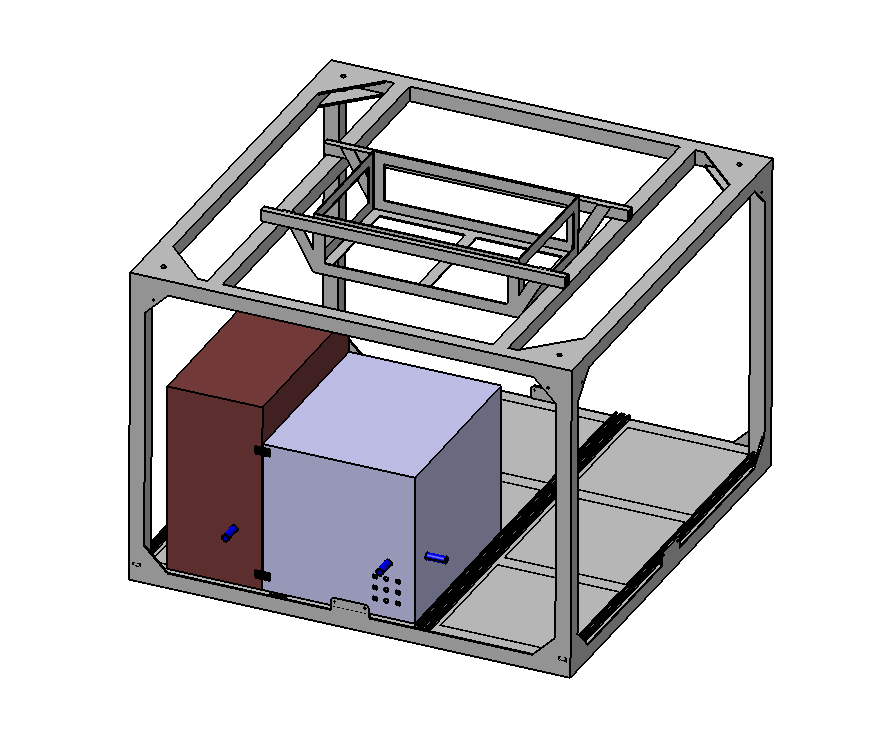
\includegraphics[width=0.7\textwidth]{6-launch-campaign-preparation/img/gondola_overview_sample.png}
    \caption{Example of Experiment Box Accommodation Inside the Gondola}
    \label{goldola_accommodation}
\end{figure}